%%% Document Author: J Moss
%%% Parts in LaTeX: Nicholas Dart
%%% Other Content: See authors list
%%% Document Last edit: 28.10.2014

\documentclass[11pt, article]{article}
\usepackage{a4wide}
\usepackage[english]{babel}
\usepackage{graphicx}
\usepackage{tabu}
\usepackage{textcomp}
\usepackage{fancyhdr}
\usepackage{lastpage}
\usepackage{titlesec}
\usepackage{lscape}

%%%%%%
%% Variables for version and release status
%% useage: \version
%%%%%%
\newcommand\version{Max Atkins}
\newcommand\release{CS22310 Assignment}
\newcommand\titleText{North Ceredigion Fitness Website Prototype Development}
\newcommand\reference{CS22310 Assignment}

%%%%%%
%% Alias
%%%%%%
\newcommand{\sectionbreak}{\clearpage} 	%% Allways start a section on a new page

\title{ \huge CS22310 - User Centred Design and Human Computer Interaction\\ \Large \titleText}
\author{
	\vspace{100pt}
	\begin{tabular}{ r || l }
		Author 	& Max Atkins \\
						& \\
		Date Published  & \today \\
						&\\
		Department		& Computer Science \\
						&\\
		Address			& Aberystwyth University \\
						& Penglais Campas \\
						& Ceredigion \\
						& SY23 3DB \\
	\end{tabular} \\
	Copyright \textcopyright Aberystwyth University 2015
	%get rid of the date on the titlepage
	\date{}
}

\pagestyle{fancy}
\fancyhf{}
\rhead{\version}
\lhead{\release}
\rfoot{Page \thepage \hspace{1pt} of \pageref{LastPage}}
\lfoot{Aberystwyth University - Computer Science}

\begin{document}
	\setcounter{page}{1}

	\maketitle

	\tableofcontents

	\section{Introduction}
		%%\input{foo/bar.tex}

	\section{Task Analysis}
	
	\subsection{Who is Involved}
	
		\begin{figure}[ht!]
	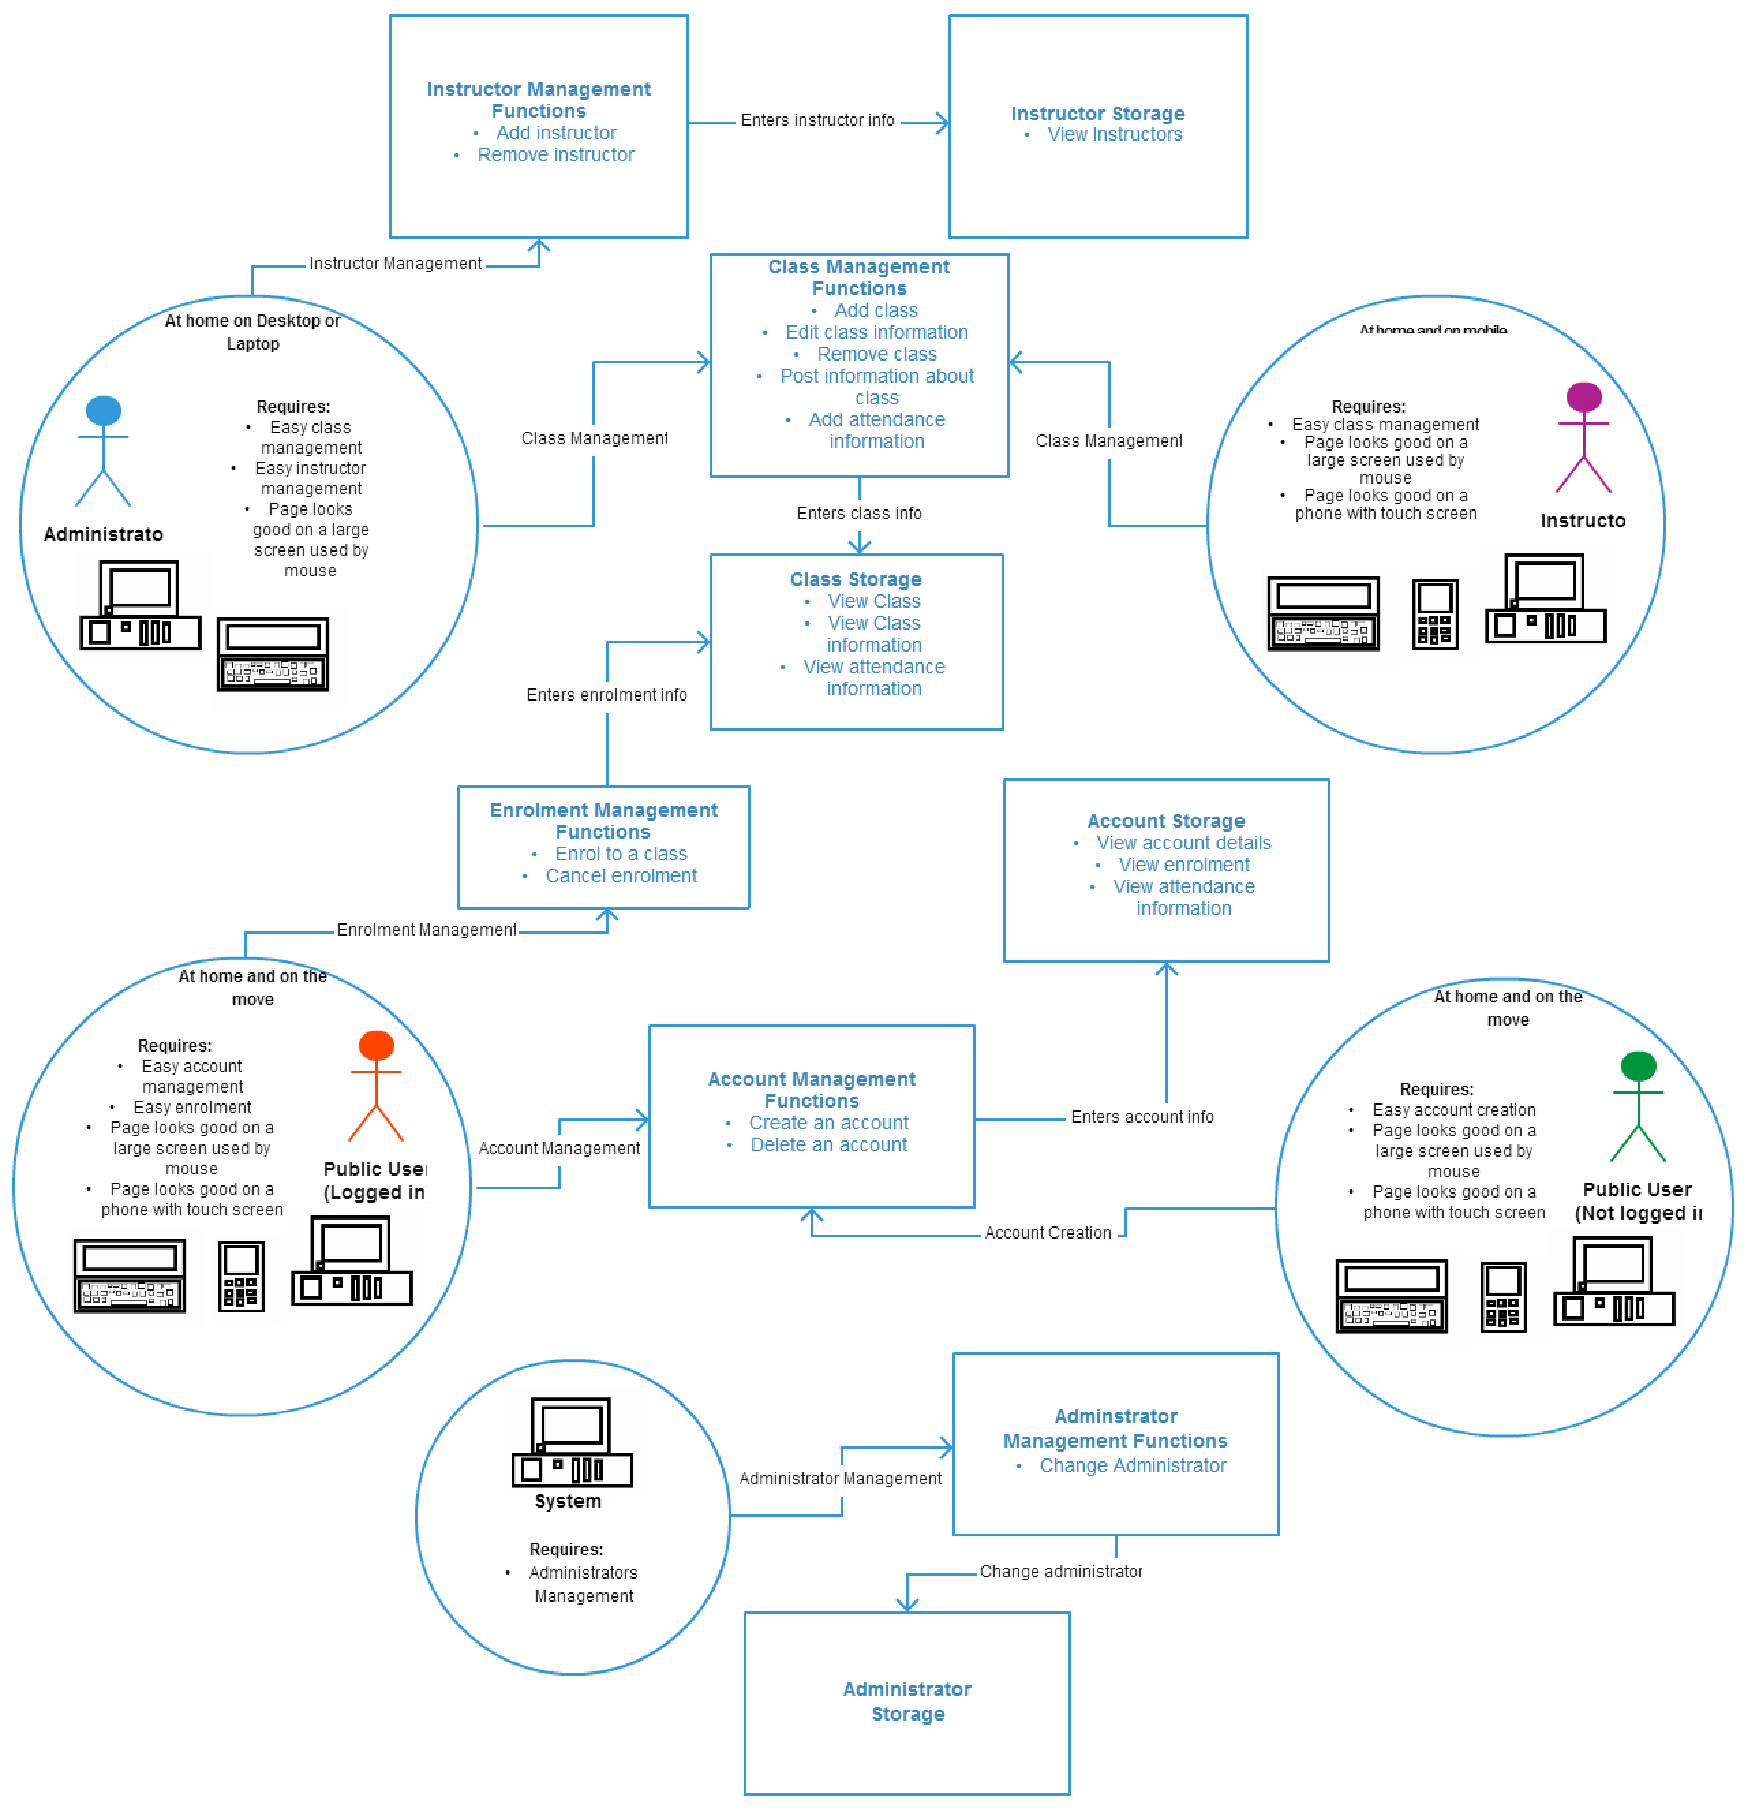
\includegraphics[scale=0.55]{images/richpicture}
 	\caption{Rich Picture}
	\end{figure}
	
	\newpage
	
	\subsection{Tasks the System Performs}
	
	\begin{figure}[ht!]
	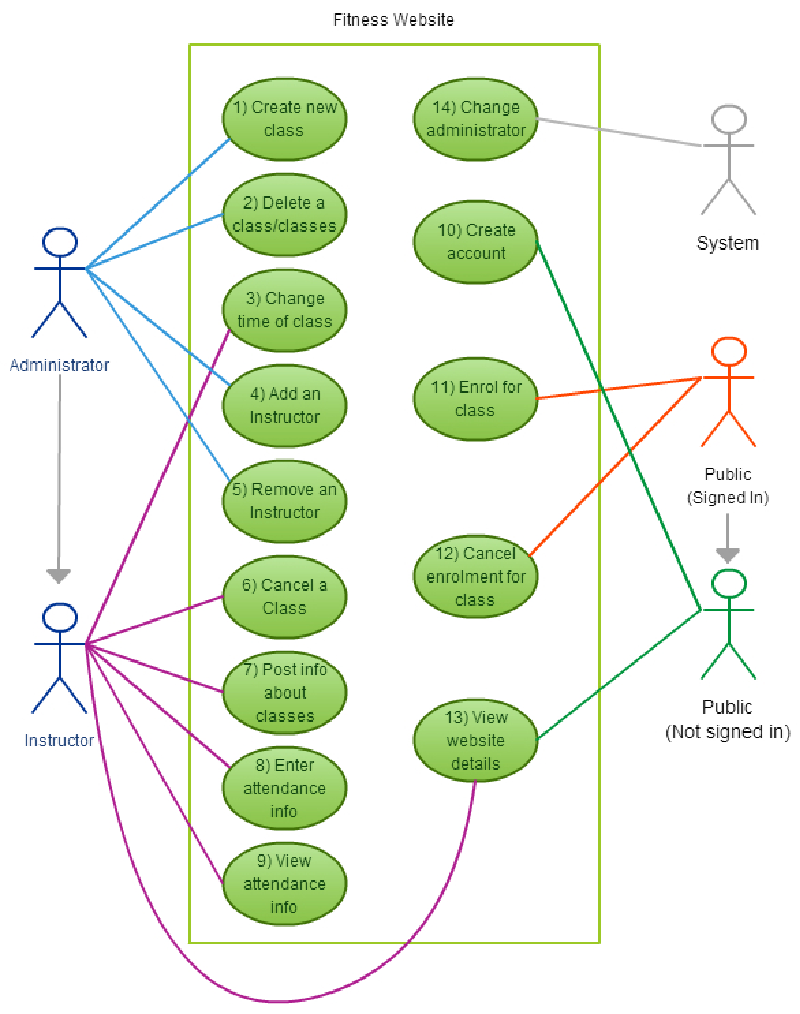
\includegraphics[scale=1]{images/usecase}
 	\caption{Use-Case Diagram}
	\end{figure}
	
	\newpage
	
	\subsection{How Tasks and Data Relate}
	
		\begin{figure}[ht!]
	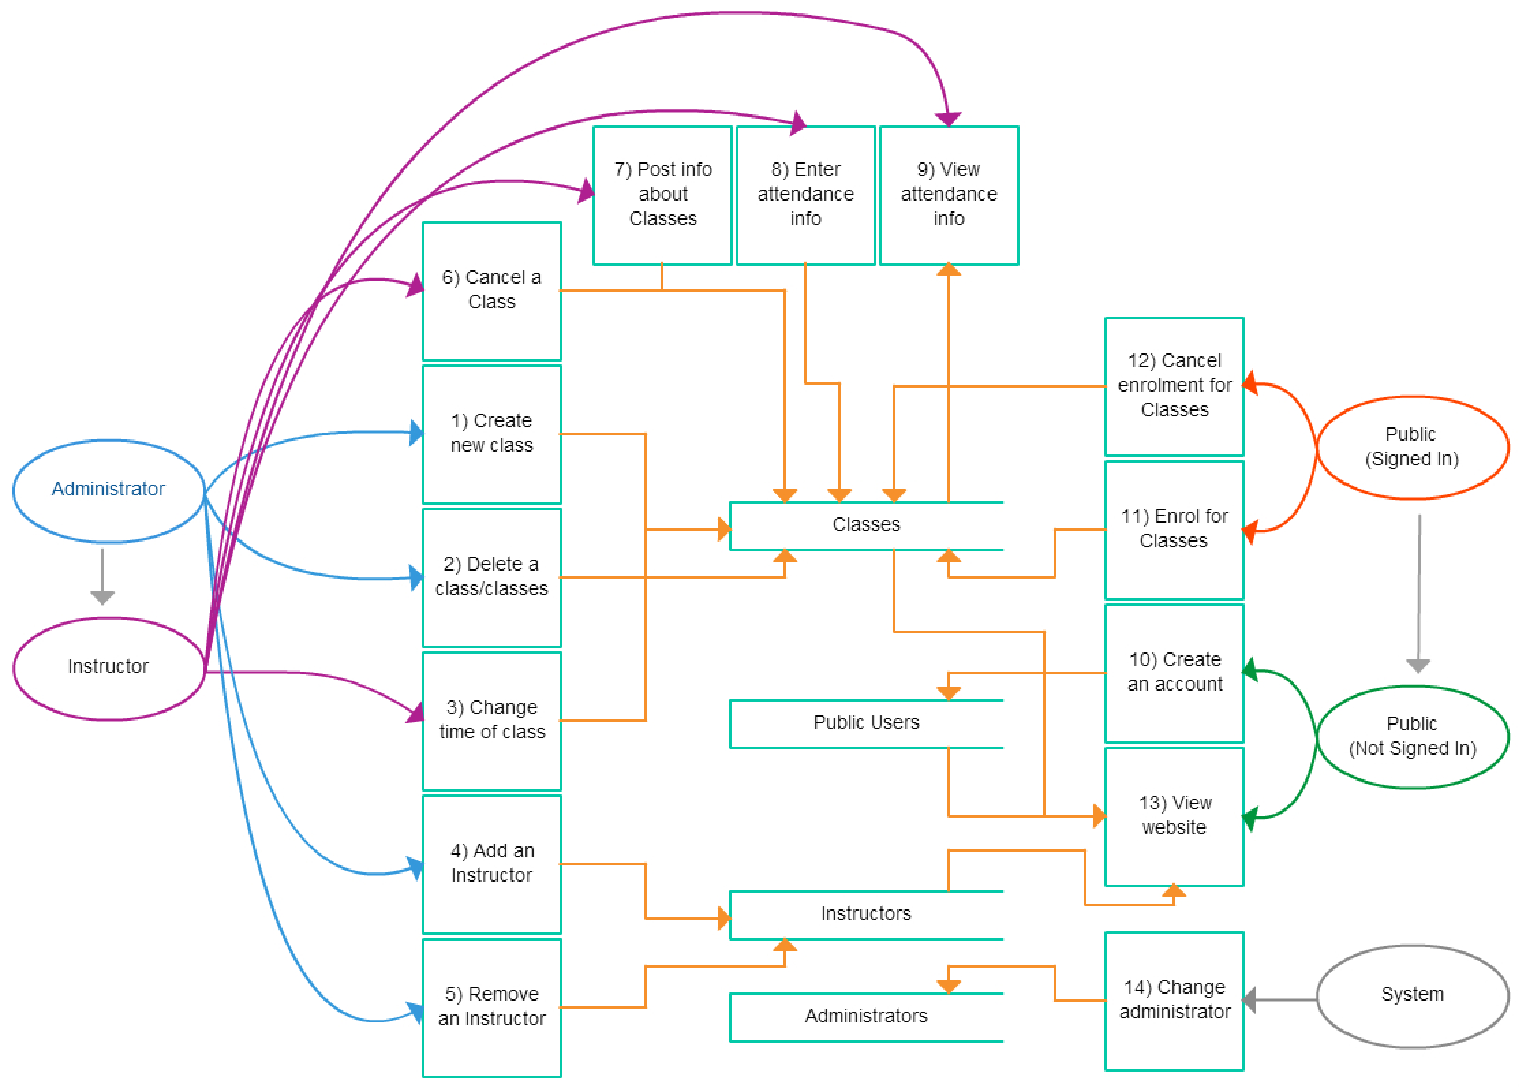
\includegraphics[scale=0.6]{images/dataflow}
 	\caption{Dataflow Diagram}
	\end{figure}
	
	\newpage
	\subsection{How Tasks are Related}
	
			\begin{figure}[ht!]
	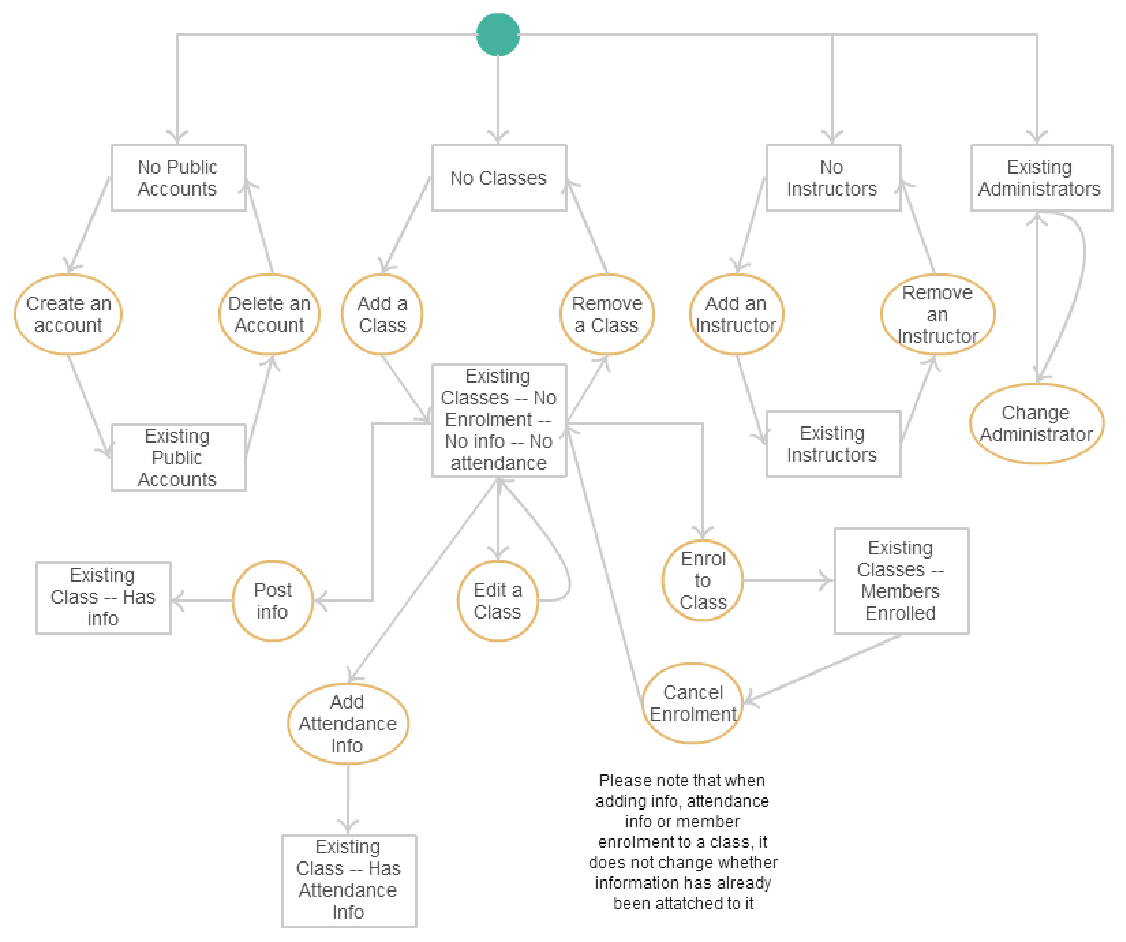
\includegraphics[scale=0.8]{images/statediagram}
 	\caption{State Transition Diagram}
	\end{figure}
	
	\section{High-Level Design}

	\subsection{Style of Interaction}

	

	\subsection{Navigation}

	\subsection{Sketches of UI}

			\begin{figure}[ht!]
	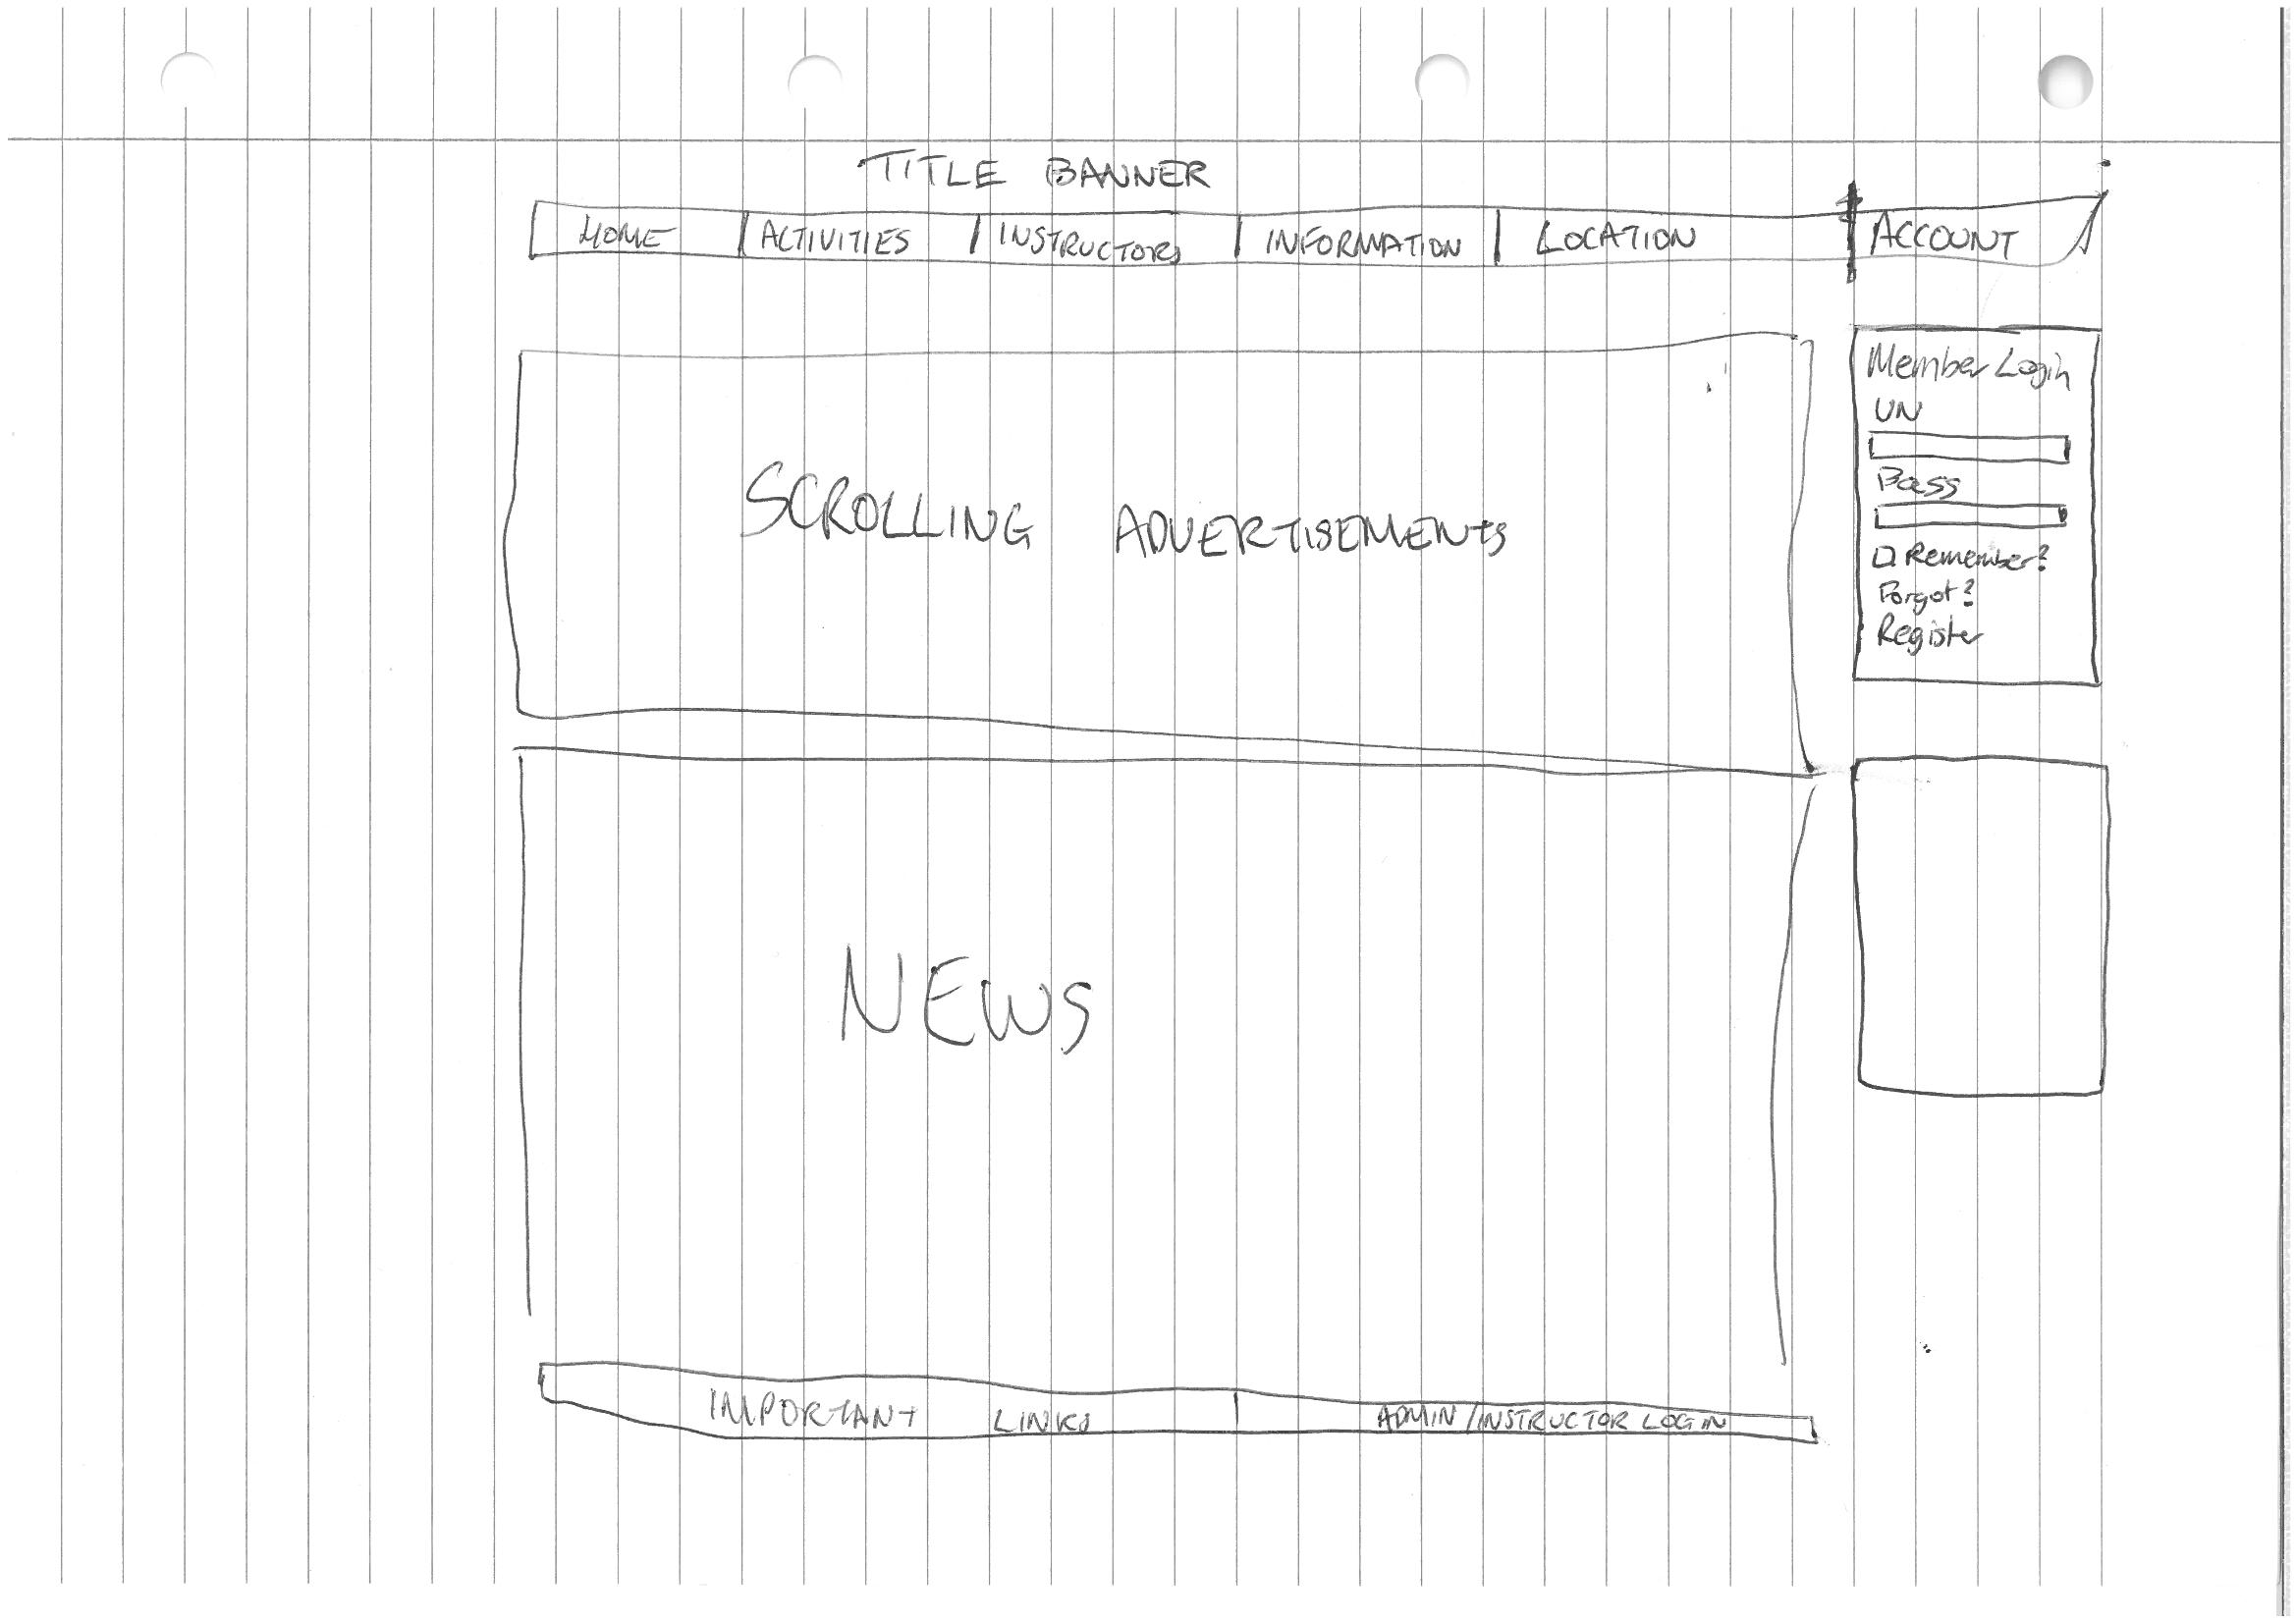
\includegraphics[scale=0.6]{images/homepage}
 	\caption{Homepage}
	\end{figure}

			\begin{figure}[ht!]
	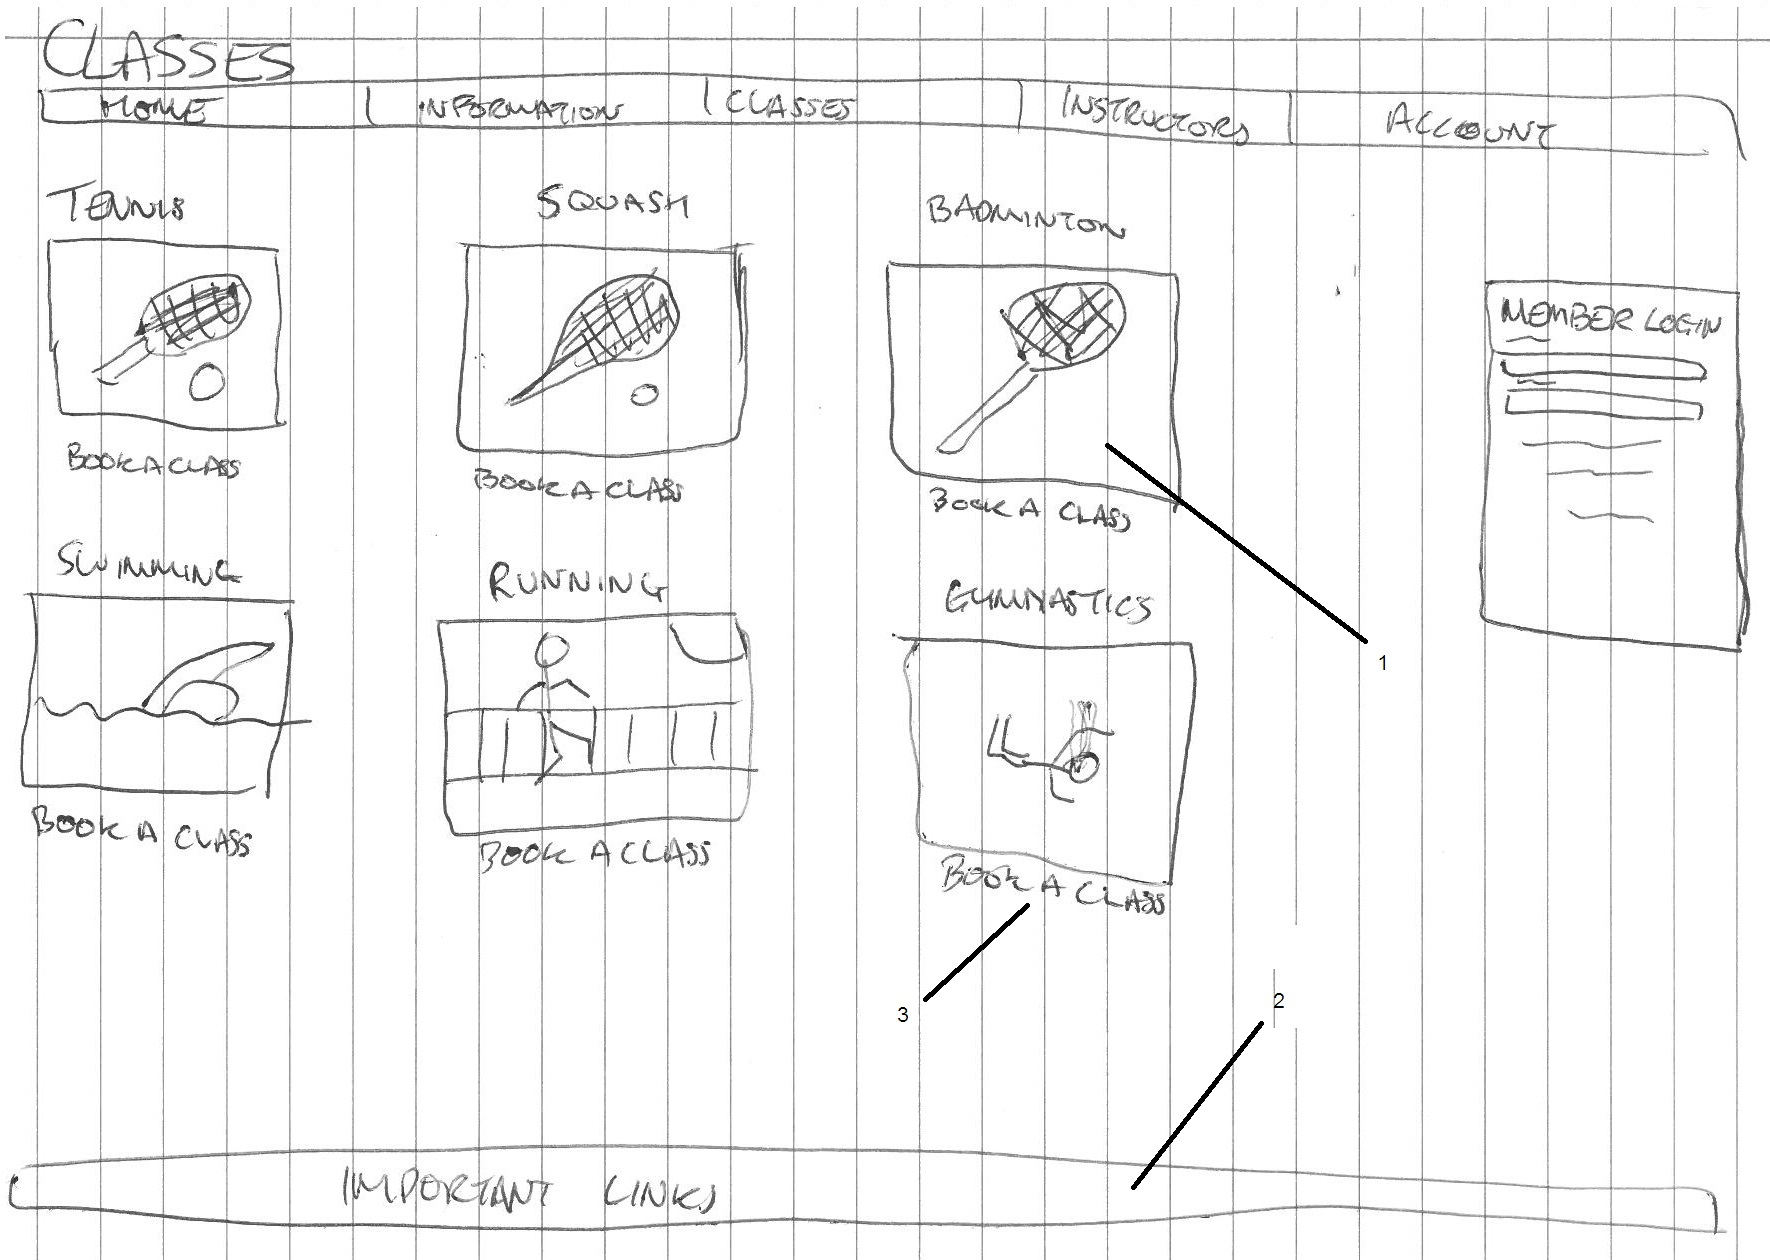
\includegraphics[scale=0.6]{images/classpage}
 	\caption{Class Listings Page}
	\end{figure}	

			\begin{figure}[ht!]
	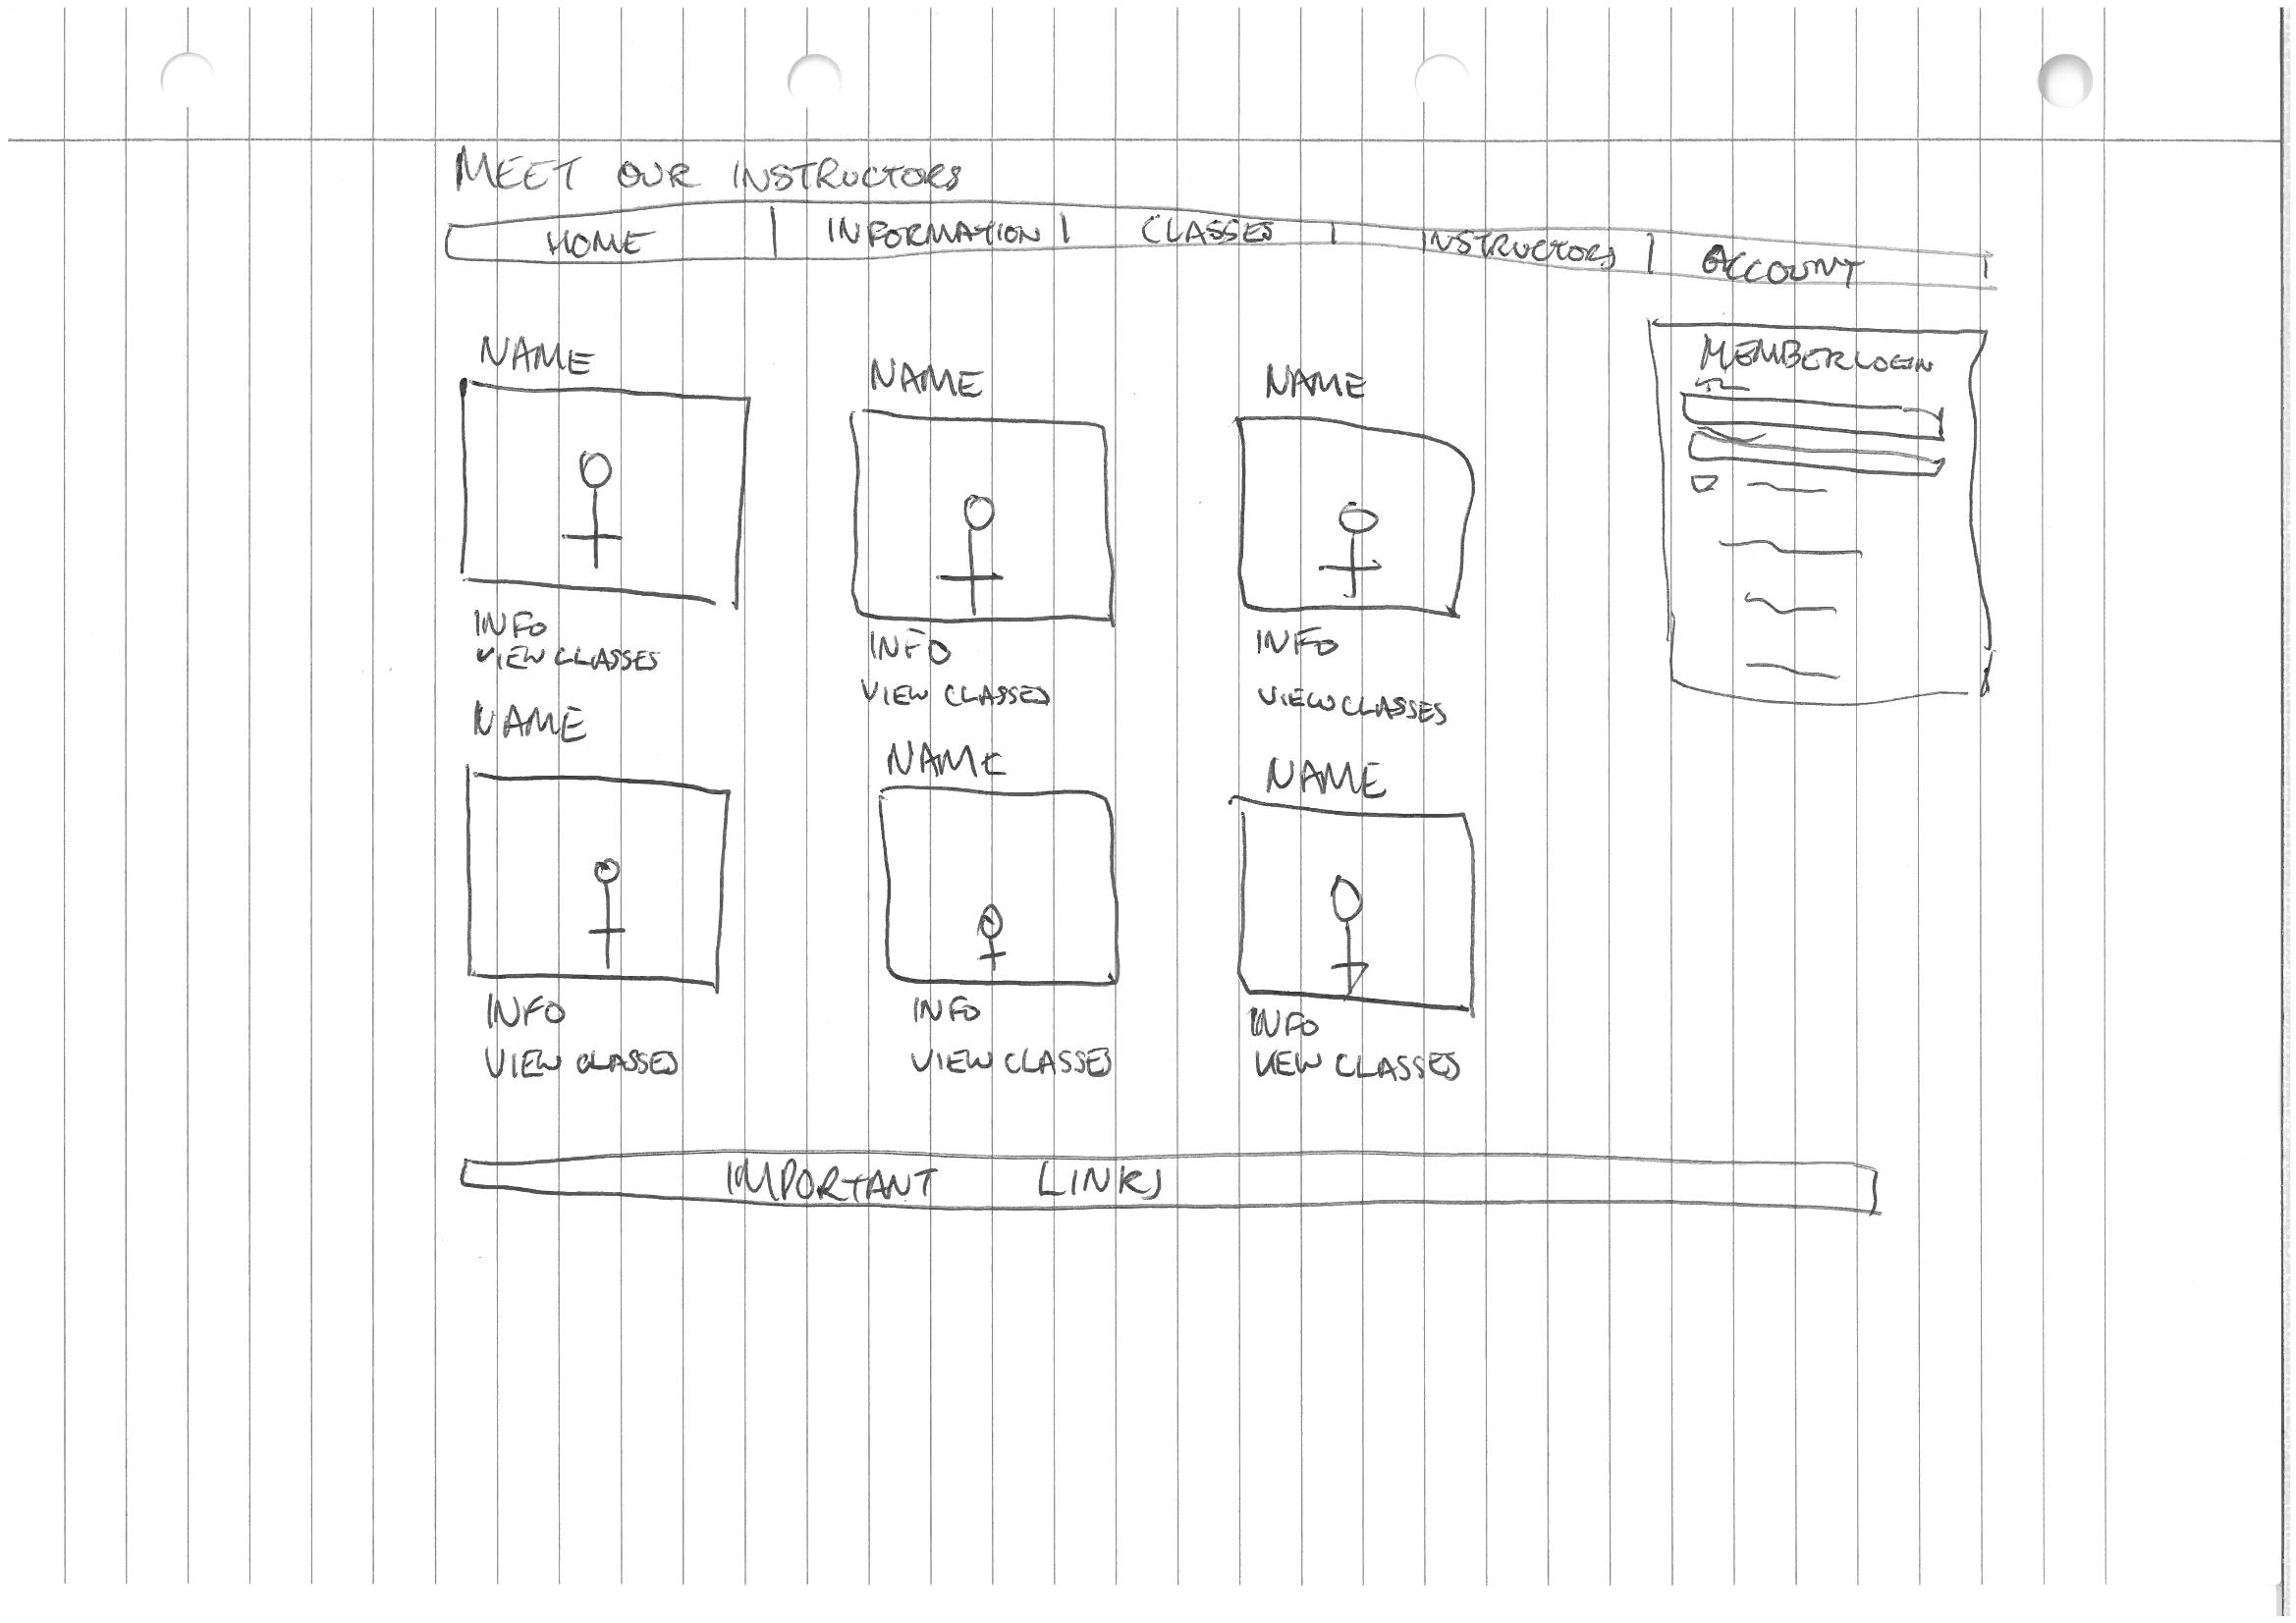
\includegraphics[scale=0.6]{images/instructorpage}
 	\caption{Instructors Listing Page}
	\end{figure}

			\begin{figure}[ht!]
	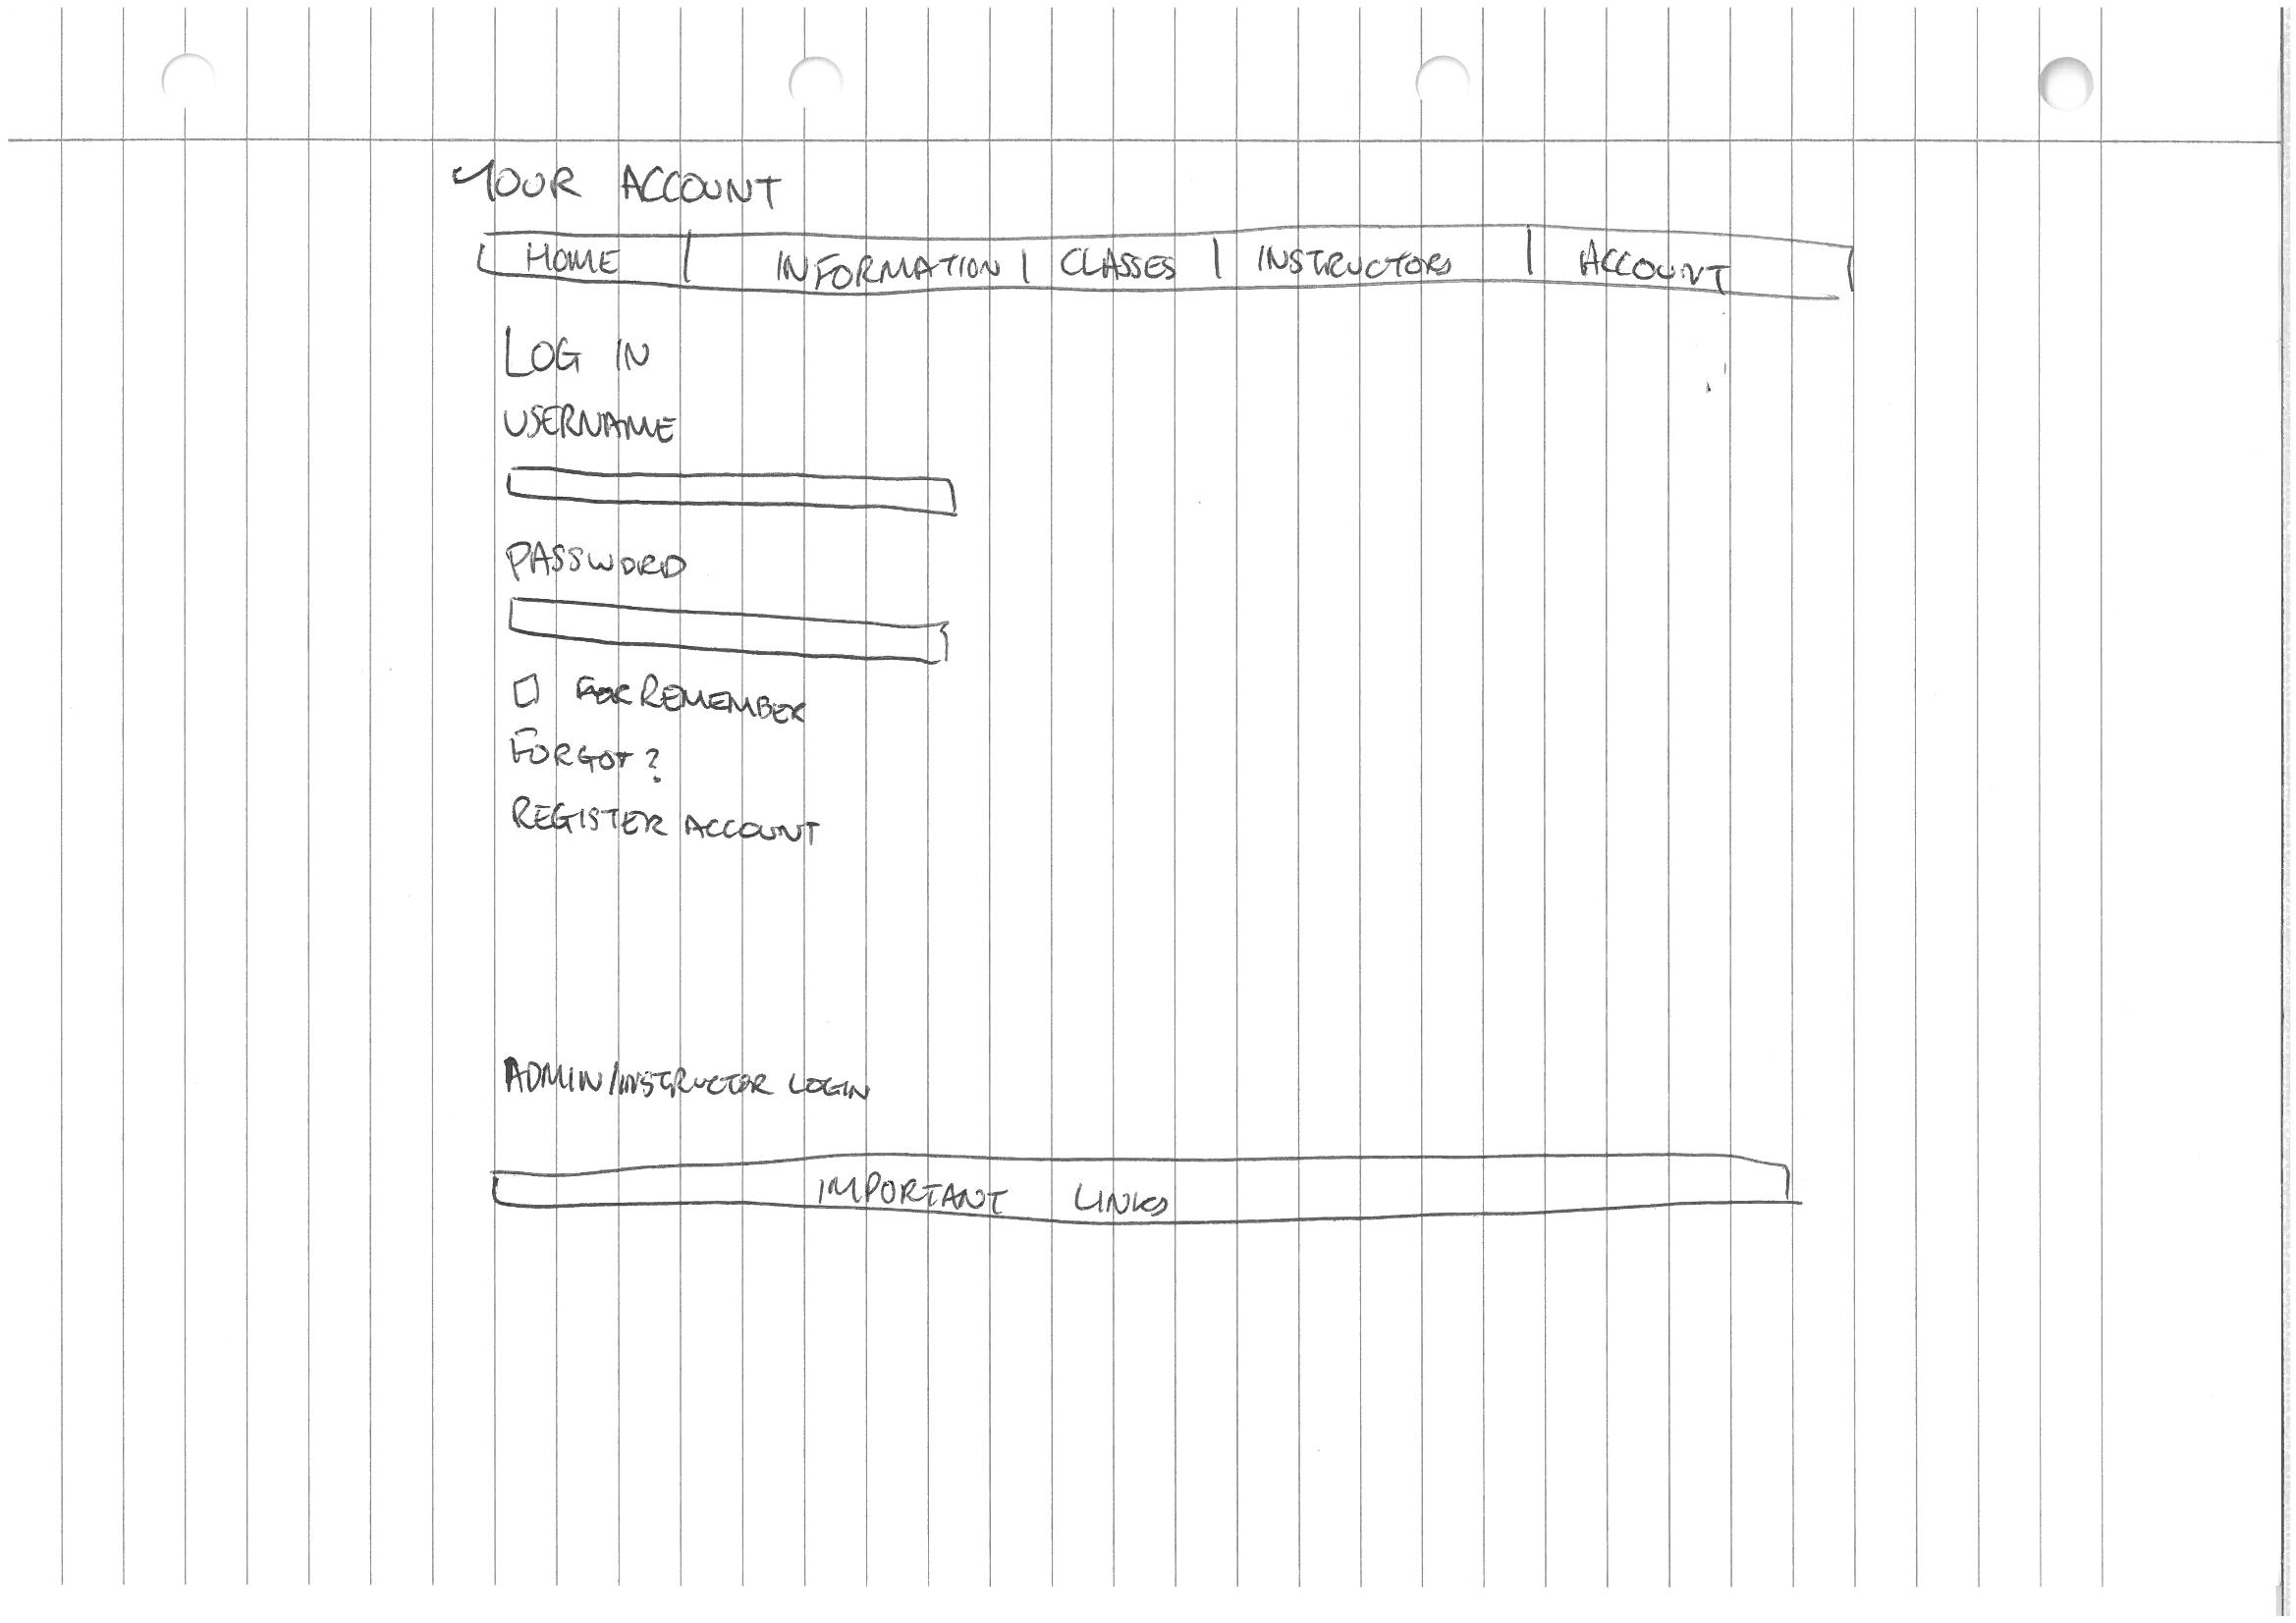
\includegraphics[scale=0.6]{images/loginpage}
 	\caption{Login Page}
	\end{figure}

			\begin{figure}[ht!]
	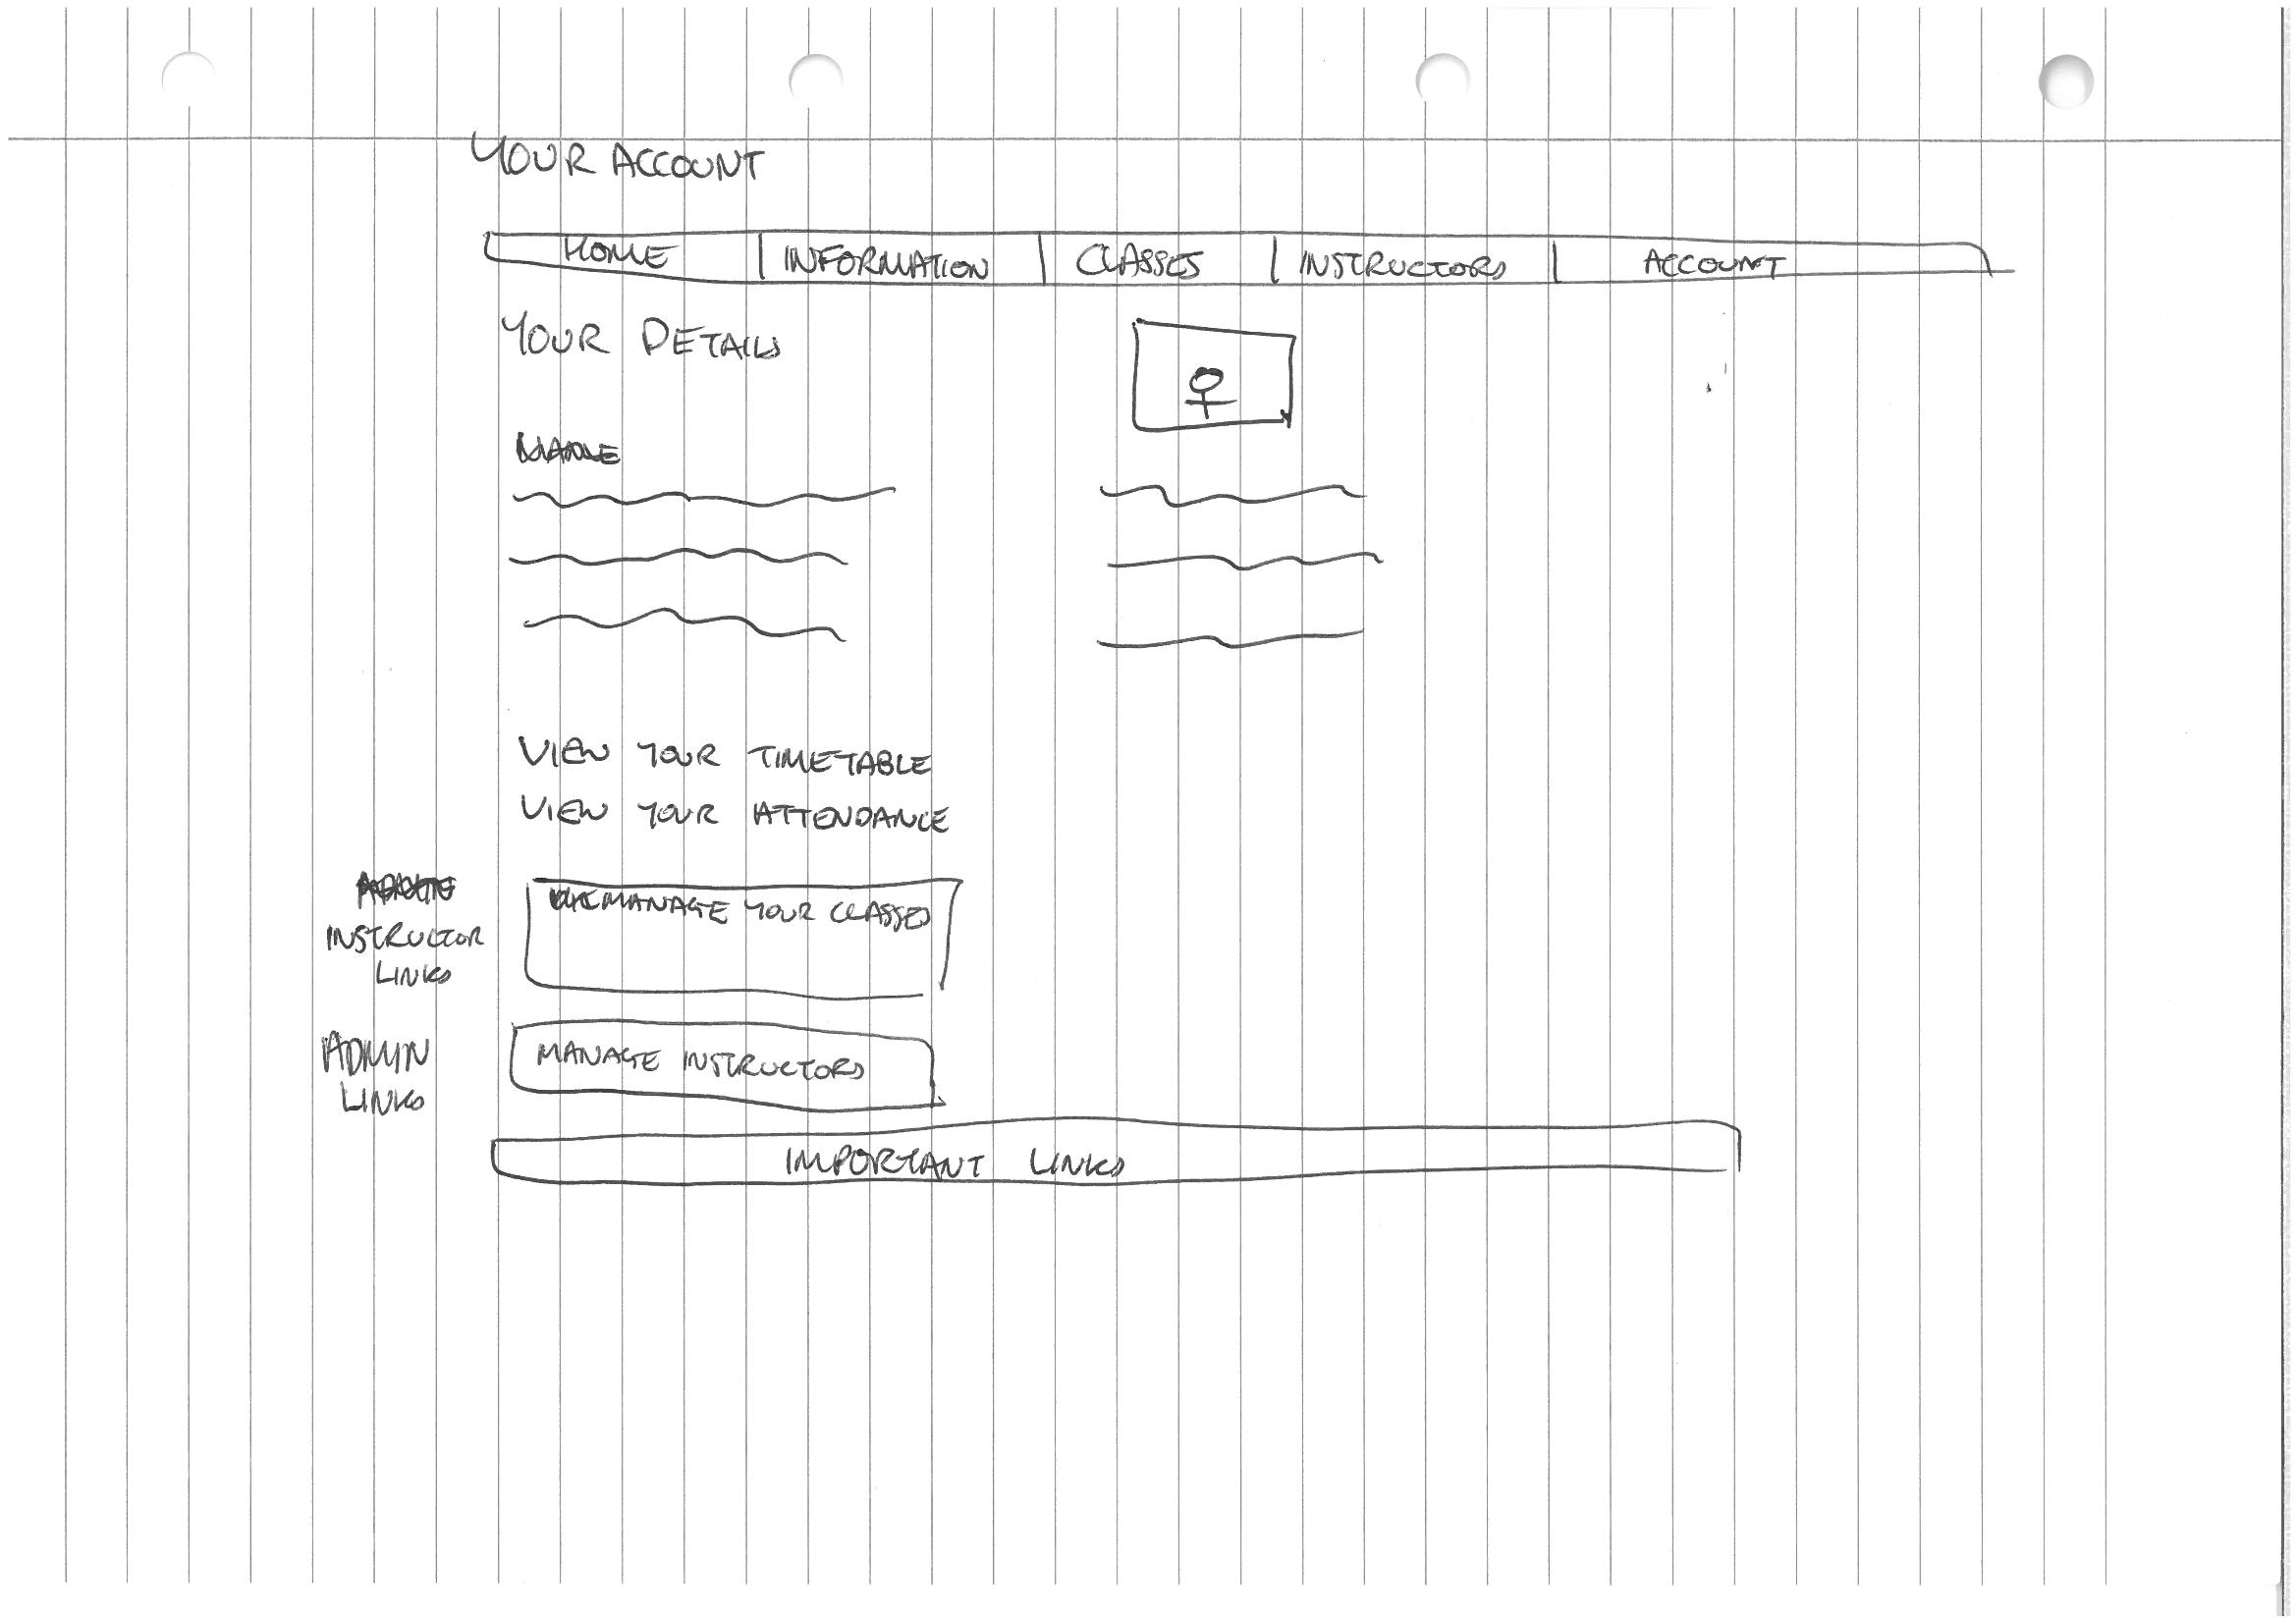
\includegraphics[scale=0.6]{images/loggedinaccpage}
 	\caption{Account Management Page}
	\end{figure}


	\section{Analysis of Prototype}


	%%\begin{landscape}

		%%\section{Bar}
			%%\input{far/foo.tex}

	%%\end{landscape}


\end{document}